% !TEX root = ../ac_paper.tex

\section{Classical Search Algorithms} \label{sec:search}
As mentioned in the previous section, breadth first search (BFS) has been applied in the past to find AC trivializations of balanced presentations. In this section, we present a greedy search (GS) algorithm. We find that this algorithm performs better than breadth-first search in finding AC trivializations of balanced presentations.
\newline 

We first recall the breadth first search algorithm. An iterative implementation of this algorithm, adapted to the problem of Andrews-Curtis conjecture, is given in \autoref{alg:bfs}. We start with an initial state, i.e. a balanced presentation for which we would like to obtain an AC trivialization, and place it in a queue. At each iteration, a state is removed from the queue and its neighbors are added if they haven't already been visited. This continues until the sought-after state, i.e. a trivial balanced presentation is found, or a maximum number of states $N$ is visited. In our experiments, we set $N=10^6$. 
\newline 

\begin{algorithm}
\caption{Breadth-First Search Algorithm}\label{alg:bfs}
\begin{algorithmic}[1] % The number [1] ensures lines are numbered
\State \textbf{Input:} A balanced presentation $\pi$, maximum number of states to visit $N$
\State \textbf{Output:} Boolean for whether an AC trivialization is found
\State Initialize a queue $Q$ and enqueue the starting node $\pi$
\State Mark $\pi$ as visited
\While{Number of visited states is less than $N$}
    \State $u \gets Q$.dequeue() \Comment{Remove the front node of $Q$}
    \For{each neighbor $v$ of $u$}
        \If{$v$ is a trivial state}
            \State \Return True \Comment{Return True if $v$ is a trivial state}
        \EndIf
        \If{$v$ has not been visited}
            \State Mark $v$ as visited
            \State $Q$.enqueue($v$) \Comment{Add $v$ to the queue}
        \EndIf
    \EndFor
\EndWhile
\State \Return False \Comment{Return False if no trivial state is found}
\end{algorithmic}
\end{algorithm}

The greedy search algorithm, \autoref{alg:gs}, differs only slightly from the breadth first search algorithm in implementation. We replace the queue with a priority queue, which stores the states in the order determined by a tuple of values: $(k, l)$ where $k$ is the total length of the presentation and $l$ is the path length between the state and the initial state. Instead of dequeuing the earliest state, the algorithm dequeues the state with the smallest value of $k$. If there is more than one state in the priority queue with the same value of $k$, the state with the smallest value of $l$ is chosen. 
\newline 

\begin{algorithm}
\caption{Greedy Search Algorithm}\label{alg:gs}
\begin{algorithmic}[1] % The number [1] ensures lines are numbered
\State \textbf{Input:} A balanced presentation $\pi$ of total length $k$, maximum number of states to visit $N$
\State \textbf{Output:} Boolean for whether an AC trivialization is found
\State Initialize a \textit{priority} queue $Q$ ordered by $(k, l)$ and enqueue the starting node $\pi$. $l$ is the length of the path connecting $\pi$ to the current node.
\State Mark $\pi$ as visited
\While{Number of visited states is less than $N$}
    \State $u \gets Q$.dequeue() \Comment{Remove the front node of $Q$}
    \For{each neighbor $v$ of $u$}
        \If{$v$ is a trivial state}
            \State \Return True \Comment{Return True if $v$ is a trivial state}
        \EndIf
        \If{$v$ has not been visited}
            \State Mark $v$ as visited
            \State $Q$.enqueue($v$) \Comment{Add $v$ to the queue}
        \EndIf
    \EndFor
\EndWhile
\State \Return False \Comment{Return False if no trivial state is found}
\end{algorithmic}
\end{algorithm}

We find that greedy-search algorithm outperforms the breadth first search algorithm in the task of solving the presentations of Miller-Schupp series \autoref{fig:performance}. Out of 1190 presentations of the Miller-Schupp series with $n, \ \text{length}(w) \leq 7$, greedy search solved 533 while BFS solved only 278 presentations. Each algorithm was constrained to visit a maximum of 1 million nodes. The percentage of presentations solved by these algorithms decreases monotonically as a function of $n$. Remarkably, however, greedy search solved all presentations with $n=1$ or total length less than 14 successfully. There are six presentations of length 14 that greedy search could not solve. We checked that four of these,
\[
\angles{x, y \mid x^{-1} y^2 x = y^{3} , x = x^{-2} y^{-1} x^2 y^{\pm 1}}
\]
\[
\angles{x, y \mid x^{-1} y^3 x = y^{4} , x = y^{\pm 1} x^2 y^{\pm 1}}
\]
are AC-equivalent to $\AK(3)$, while the other two
\[
\angles{x, y \mid x^{-1} y^2 x = y^{3} , x = y x^2 y^{\pm 1} x^{-2}}
\]
could be related neither to $\AK(3)$ nor to the trivial presentation with any sequence of moves that allowed the length of each relator to increase up to 20. 
\newline 

For presentations solved by greedy search, we plot the maximum amount by which the total length of a presentation increased in an AC trivialization path in \autoref{fig:gs_length_increase}. In most cases, there was no increase in length; and the maximum increase was only 5. This seemed surprising to us at first given that we allowed the relator lengths to increase by a much larger number in our search process. 
\footnote{The length of each relator was allowed to increase up to \(2 \times \text{max}(2n+3, \text{length}(w)+1) + 2\), which is twice the maximum of the initial lengths of the two relators in a presentation, plus an additional 2. 
The maximum possible increase in presentation length is twice this number minus the original length. For $n, \ \text{length}(w) \leq 7$, this value lies in the range $[17, 53]$. 
} 
However, the hard cutoff set by visiting a maximum of only 1 million nodes ensures that any presentation that needs to be mapped to a much longer presentation before it is trivialized would remain unsolved by the greedy search algorithm. This limitation could be cured either by increasing the number of maximum nodes (at the cost of more memory) or by using a different criterion to order nodes in the priority queue. It will be useful to explore the latter approach perhaps by looking for a criterion itself using deep learning algorithms.
\newline

We also plot the lengths of AC sequences discovered by greedy search as functions of $n$ and the maximum increase in the presentation length (\autoref{fig:gs_path_length}). Unsurprisingly, path lengths increase proportionally with the increase in the total length of the presentation (\autoref{fig:path_lengths_vs_length_increase}). 
The following presentation with $n=5$ had the longest AC trivialization path,
\[
\angles{x^{-1} y^5 x = y^6 \mid  x = y x^2 y^{-1}}
\]
requiring a sequence of 344 AC moves. Note that greedy search does not necessarily find the shortest paths of trivialization. We will see in \autoref{sec:application} that a Reinforcement Learning algorithm finds shorter trivializing sequences for many examples of the Miller-Schupp series. This again hints at the potential utility of exploring more efficient critera for ordering nodes in the priority queue.  
	
\begin{figure}
	\centering
	\begin{subfigure}[b]{0.5\textwidth}
		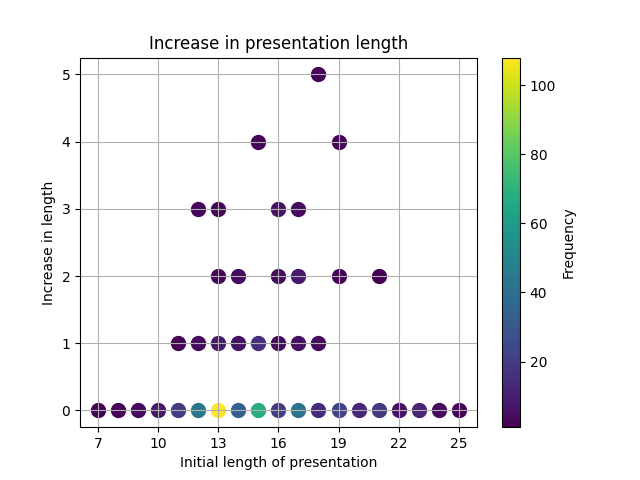
\includegraphics[width=\textwidth]{fig/gs_length_increase_vs_length.png}
		\caption{Distribution versus initial presentation length}
		\label{fig:gs_length_increase_vs_length}
	\end{subfigure}%
	%add desired spacing between images, e. g. ~, \quad, \qquad etc.
	%(or a blank line to force the subfigure onto a new line)
	\begin{subfigure}[b]{0.5\textwidth}
		\centering
		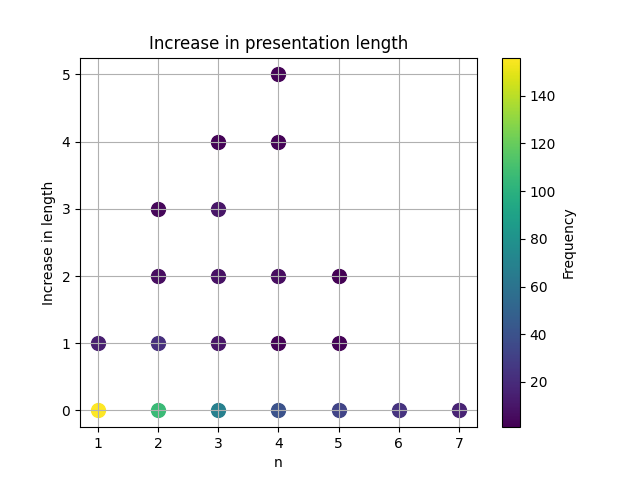
\includegraphics[width=1.1\textwidth]{fig/gs_length_increase_vs_n.png}
		\caption{Distribution versus $n$}
		\label{fig:gs_length_increase_vs_n}
	\end{subfigure}
	\caption{
This figure illustrates the maximum increase in the length of a presentation relative to its initial length along the AC trivialization path. The increase is plotted as a function of the initial length of the presentation on the left and as a function of $n$ on the right.} \label{fig:gs_length_increase}
\end{figure}


\begin{figure}
	\centering
	\begin{subfigure}[b]{0.4\textwidth}
		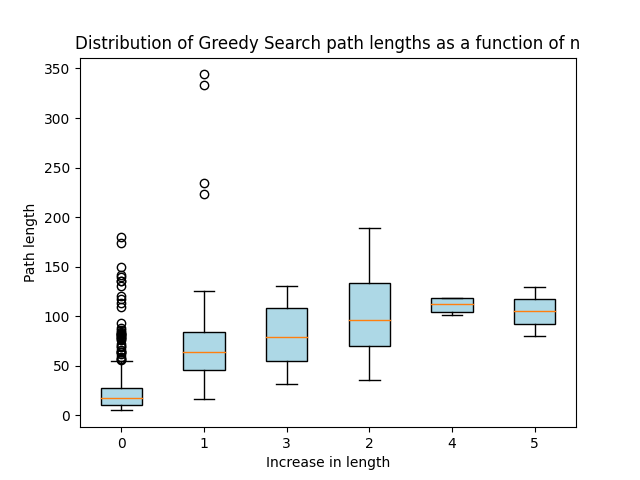
\includegraphics[width=\textwidth]{fig/path_lengths_vs_length_increase.png}
		\caption{Distribution versus initial presentation length}
		\label{fig:path_lengths_vs_length_increase}
	\end{subfigure}
	\begin{subfigure}[b]{0.4\textwidth}
	\centering
		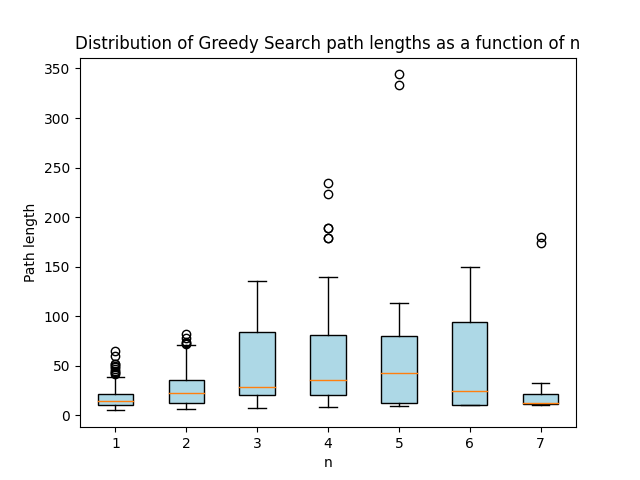
\includegraphics[width=1.1\textwidth]{fig/gs_path_lengths.png}
		\caption{Distribution versus $n$}
		\label{fig:gs_path_lengths}
	\end{subfigure}%
	\caption{Distribution of lengths of AC-trivialization paths learned by greedy search as a function of maximum increase in presentation length (left) and $n$ (right).} \label{fig:gs_path_length}
\end{figure}

\subsection{The Stable Andrews-Curtis Conjecture}
We applied the greedy and breadth first search algorithms to trivialize the length 25 presentation mentioned in \autoref{sec:stable_ac},
\[
\angles{ x, y \mid 
x^{-1}y^{-1}xy^{-1}x^{-1}yxy^{-2}xyx^{-1}y, 
y^{-1}x^{-1}y^2x^{-1}y^{-1}xyxy^{-2}x }.
\]
We placed a cutoff of a maximum of 1 million nodes to visit for each of our search algorithms and allowed the length of each relator to increase up to $15$. Greedy search found a path connecting this presentation to $\AK(3)$, while breadth first search could only reduce the presentation length to $14$. 
\footnote{We repeated the search process with breadth first search with a cutoff of 5 million nodes. It failed to reduce the presentation length any further.}
The sequence of moves discovered by greedy search is given in \autoref{sec:stable_ak3}.

\subsection{Limitations}. While greedy search algorithm performs better than breadth first search, it has some of the same limitations. Namely, it is memory inefficient, and we cannot leverage the parallelizability of modern hardware architectures. It also does not learn a general algorithm that would find an AC trivialization for any given balanced presentation. A simple candidate for algorithms that do not have these downsides are reinforcement learning algorithms. In particular, the policy gradient algorithms, which we will review in \autoref{sec:rl} are memory efficient and can be trained in a highly distributed manner. In this paper, we trained these learning algorithms with limited computation power but noticed that they easily outperform breadth first search and often find shorter sequences of AC moves compared to the greedy search when they solve a presentation. 
